
%----------------------------------------------------------------------------------------
%	PACKAGES AND THEMES
%----------------------------------------------------------------------------------------

\documentclass[aspectratio=169]{beamer}
\mode<presentation> {
	
	\usetheme{Boadilla}
}
\usepackage{xcolor}
\definecolor{lmugreen}{RGB}{0, 136, 58}
\usecolortheme[named=lmugreen]{structure}
\definecolor{pastelBlue}{RGB}{102,153,204}   % soft blue
\definecolor{pastelRed}{RGB}{204,102,102}    % soft red
\usepackage{graphicx} % Allows including images
\usepackage{booktabs} % Allows the use of \toprule, \midrule and \bottomrule in tables
\usepackage[english]{babel}
\usepackage[utf8]{inputenc}
\usepackage{amsmath,amssymb} % math symbols
\usepackage{graphicx}
\usepackage{float}
\usepackage{hyperref} % for URLs
\newcommand{\gray}{\rowcolor[gray]{.90}}
\usepackage{verbatim}
\usepackage{textpos} % logo position
\usepackage[default]{sourcesanspro} % font type
\usepackage{cases} % math cases
\usepackage{tikz}
\usetikzlibrary{arrows.meta, positioning, shapes}
% Put this in your preamble:

% Caption
\usepackage{caption}
\DeclareCaptionFont{tiny}{\tiny}
\captionsetup{font=scriptsize,labelfont=scriptsize,justification=centering}

% ToC
\AtBeginSection[]{
	\begin{frame}[noframenumbering, plain]
	\frametitle{Outline}
	\setcounter{tocdepth}{1}
	\tableofcontents[currentsection]
\end{frame}
}

% Remove navigation 
\beamertemplatenavigationsymbolsempty

% R 
\usepackage{listings}
\lstset{
language=R,
basicstyle=\scriptsize\ttfamily,
commentstyle=\ttfamily\color{gray},
backgroundcolor=\color{white},
showspaces=false,
showstringspaces=false,
showtabs=false,
tabsize=2,
captionpos=b,
breaklines=false,
breakatwhitespace=false,
title=\lstname,
escapeinside={},
keywordstyle={},
morekeywords={}, 
belowskip = -1.2 \baselineskip,
}

%----------------------------------------------------------------------------------------
%	TITLE PAGE
%----------------------------------------------------------------------------------------

\addtobeamertemplate{frametitle}{}{%
	\begin{textblock*}{100mm}(0.88\textwidth,-0.5cm)
		\includegraphics[height=1cm,width=2cm]{lmu_logo}
\end{textblock*}}

%\includegraphics[width=0.3\textwidth]{lmu_logo}
\vspace*{-1cm}

\title{Functional ANOVA Decomposition} 

\author{Juliet Fleischer} 
\institute[LMU]{LMU} % Your institution as it will appear on the bottom of every slide, may be shorthand to save space
{

}
\begin{document}

{
\usebackgroundtemplate{\includegraphics[width=\paperwidth]{lmu-background.pdf}}
\begin{frame}
\begin{columns}
	\begin{column}{0.4\textwidth}
		\vspace{3cm}
		
		\textbf{\textcolor{white}{Functional ANOVA Decomposition}}\\
		\vspace{1cm}

		\textcolor{white}{\footnotesize Juliet Fleischer \\
			\today}
	\end{column}
	\begin{column}{0.49\textwidth}
		\vspace{2cm}
		\begin{center}
			\includegraphics[width=1\textwidth]{../images/experiment_section/mixed_a1p20_a2p20_a11m10_a22p10_a12p00_rhop00_main.png}
		\end{center}
	\end{column}
\end{columns}
\end{frame}
}
%----------------------------------------------------------------------------------------
%	PRESENTATION SLIDES
%----------------------------------------------------------------------------------------


\section{Research Context}

\begin{frame}{Overview of the fANOVA Research Field}
\centering
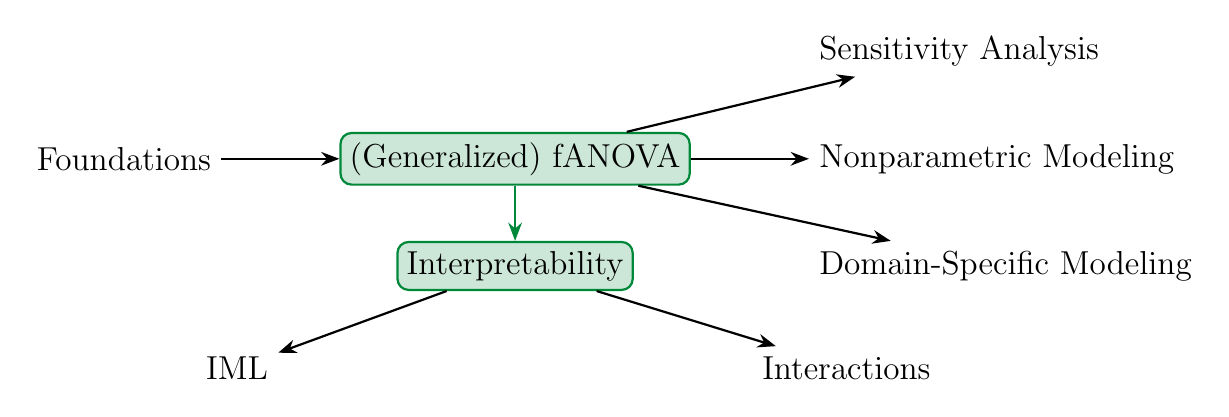
\begin{tikzpicture}[
    node distance=0.7cm and 1.5cm,
    every node/.style={font=\large},
    >=Stealth, thick
]

% Nodes
\node (foundations) {Foundations};
\node[right=of foundations, draw=lmugreen, fill=lmugreen!20, rounded corners] (fanova) {(Generalized) fANOVA};
\node[above right=of fanova] (sensitivity) {Sensitivity Analysis};
\node[right=of fanova] (nonparam) {Nonparametric Modeling};
\node[below right=of fanova] (domain) {Domain-Specific Modeling};
\node[below=of fanova, draw=lmugreen, fill=lmugreen!20, rounded corners] (interpret) {Interpretability};
\node[below left=of interpret] (iml) {IML};
\node[below right=of interpret] (interactions) {Interactions};

% Arrows
\draw[->] (foundations) -- (fanova);
\draw[->] (fanova) -- (sensitivity);
\draw[->] (fanova) -- (nonparam);
\draw[->] (fanova) -- (domain);
\draw[->, color = lmugreen] (fanova) -- (interpret);
\draw[->] (interpret) -- (iml);
\draw[->] (interpret) -- (interactions);

\end{tikzpicture}

\end{frame}





\section{Classical fANOVA}
% \begin{frame}{Formal Setting}
%   \begin{itemize}
%     \item measure space, probability measure, random vector, subvector, complementary vector, pdf
%     \item measure space of square integrable functions
%     \item inner product
%     \item norm
%   \end{itemize}
  
% \end{frame}

\begin{frame}{Decomposition of Model into Interpretable Components} % What is it?
\begin{block}{General Form}
\[
  \begin{aligned}
    y(\boldsymbol{X}) 
    &= \sum_{u \subseteq \{1,\dots,N\}} y_{u}(\boldsymbol{X}_u) \\[3pt]
    &\uncover<3->{= y_{\emptyset} 
       + \big( y_{\{1\}}(X_1) + \dots + y_{\{N\}}(X_N) \big)} \\[2pt]
    &\uncover<4->{\quad + \big( y_{\{1, 2\}}(X_1,X_2) 
                 + y_{\{1, 3\}}(X_1,X_3) + \dots \big)} \\[2pt]
    &\uncover<5->{\quad + \big( y_{\{1, 2, 3\}}(X_1,X_2,X_3) + \dots \big) 
       + \dots + y_{\{1, \dots, N\}}(X_1, \dots, X_N)}
  \end{aligned}
\]
\end{block}

\begin{itemize}
  \item<2-> $y : \text{Model}$
  \item<2-> $y_u : \text{Component functions for subvector } \boldsymbol{X}_u$
  \item<2-> $\boldsymbol{X} = (X_1, \dots, X_N)$: input variables (assumed to be independent in classical fANOVA)
\end{itemize}
\end{frame}

\begin{frame}{Conditions for Interpretability under Independent Inputs} % What conditions do we need?
  \begin{block}{Strong Annihilating Conditions}
    \[
      \int_{\mathbb{R}} y_u(\boldsymbol{x}_u) f_{\{i\}}(x_i) \, d\nu(x_i) = 0 
      \quad \text{for} \ i \in u \neq \emptyset
    \]
  \end{block}

  \begin{itemize}
    \item<2-> $f_{\{i\}}$ : marginal density of variable $X_i$
    \item<2-> $\nu$: reference measure on $\mathbb{R}$; $d\nu(x_i)$ indicates integration with respect to $\nu$ in the variable $x_i$
  \end{itemize}

  \uncover<3->{It follows:}
  \begin{align*}
    \uncover<3->{\mathbb{E}[y_u(\boldsymbol{X}_u)] = 0}
  \end{align*}
  \begin{align*}
    \uncover<4->{\mathbb{E}[y_u(\boldsymbol{X}_u) y_v(\boldsymbol{X}_v)] = 0 \quad (u \neq v)}
  \end{align*}
\end{frame}


\begin{frame}{Recursive Form of the Components}
    % y_emptyset always visible
    \[
    y_{\emptyset} = \int_{\mathbb{R}^N} y(\boldsymbol{x}) 
    \prod_{i=1}^{N} f_{\{i\}}(x_i) \, d\nu (x_i) 
    = \mathbb{E}[y(\boldsymbol{X})]
    \]

    % Single align with overlays
    \begin{align*}
        \onslide<3->{%
        y_u(\boldsymbol{X}_u) 
        &= \int_{\mathbb{R}^{N- |u|}} 
            y(\boldsymbol{X}_u, \boldsymbol{x}_{-u}) 
            \prod_{i=1, i \notin u}^{N} f_{\{i\}}(x_i) 
            \, d\nu (x_i) 
          - \sum_{v \subsetneq u} y_v(\boldsymbol{X}_v) 
        } \\[0.5em]
        \onslide<4->{%
        &= \mathbb{E}[y(\boldsymbol{X}_{u}, \boldsymbol{X}_{-u}) 
           \mid \boldsymbol{X}_u = \boldsymbol{x}_u]
           - \sum_{v \subsetneq u} y_v(\boldsymbol{X}_v)
        }
    \end{align*}

    \uncover<2->{
        \begin{itemize}
        \item \(f_{\boldsymbol{X}}(\boldsymbol{x})\,d\nu(\boldsymbol{x})
               = \prod_{i=1}^{N} f_{\{i\}}(x_i)\,d\nu(x_i)\)
        \item \(f_{\boldsymbol{X}}(\boldsymbol{x})\,d\nu (\boldsymbol{x}_{-u})
               = \prod_{i=1, i \notin u}^{N} f_{\{i\}}(x_i)\,d\nu(x_i)\)
    \end{itemize}
    }

\end{frame}



\begin{frame}{Example of Recursive Form}
  \begin{itemize}
    \item<1-> $N = 3$, $u = \emptyset$
  \end{itemize}
  \uncover<2->{
    \[
    y_{\emptyset} 
      = \int_{\mathbb{R}^3} y(\boldsymbol{x}) 
        \prod_{i=1}^{3} f_{\{i\}}(x_i) \, d\nu (x_i) 
      = \mathbb{E}[y(\boldsymbol{X})]
    \]
  }

  \begin{itemize}
    \item<3-> $u = \{1\}$ $\rightarrow$ $v \in \{\emptyset\}$
  \end{itemize}
  \uncover<4->{
    \[
    y_{\{1\}}(x_1) 
      = \int_{\mathbb{R}^{2}} 
          y(x_{1}, x_{2}, x_{3}) 
          \prod_{i=2}^{3} f_{\{i\}}(x_i) \, d\nu (x_i) 
        -  y_{\emptyset}
      = \mathbb{E}[y(X_1, X_2, X_3)|X_1 = x_1] - y_{\emptyset}
    \]
  }

    \begin{itemize}
    \item<5-> $u = \{2\}$ $\rightarrow$ $v \in \{\emptyset\}$
  \end{itemize}
  \uncover<6->{
    \[
    y_{\{2\}}(x_2) 
      = \int_{\mathbb{R}^{2}} 
          y(x_{1}, x_{2}, x_{3}) 
          \prod_{i=1, i \neq 2}^{3} f_{\{i\}}(x_i) \, d\nu (x_i) 
        -  y_{\emptyset}
      = \mathbb{E}[y(X_1, X_2, X_3)|X_2 = x_2] - y_{\emptyset}
    \]
  }
\end{frame}

\begin{frame}
    \begin{itemize}
    \item $u = \{1,2\}$ $\rightarrow$ $v \in \{\emptyset, \{1\}, \{2\}\}$
  \end{itemize}
  \uncover<2->{
    \begin{align*}
    y_{\{1,2\}}(x_1, x_2) 
      &= \int_{\mathbb{R}} 
          y(x_1, x_2, x_3) 
          f_{\{3\}}(x_3) \, d\nu (x_3) 
        -  y_{\{1\}}(x_1) -  y_{\{2\}}(x_2) - y_{\emptyset} \\[3pt]
      &= \mathbb{E}[y(X_1, X_2, X_3)|X_1 = x_1, X_2 = x_2] 
        - y_{\{1\}}(x_1) - y_{\{2\}}(x_2) - y_{\emptyset}
    \end{align*}
  }
  \begin{itemize}
      \item<3-> $u = \{1, 2, 3\}$ $\rightarrow$ $v \in \{\emptyset, \{1\}, \{2\}, \{3\}, \{1, 2\}, \{1, 3\}, \{2, 3\}\}$
  \end{itemize}
  \uncover<4->{
    \begin{align*}
    y_{\{1,2,3\}}(x_1, x_2, x_3) 
      &= y(x_1, x_2, x_3)
        -  y_{\{1\}}(x_1) -  y_{\{2\}}(x_2) - y_{\{3\}}(x_3) - y_{\emptyset} \\[3pt]
      &- y_{\{1, 2\}}(x_1, x_2) - y_{\{1, 3\}}(x_1, x_3) - y_{\{2, 3\}}(x_2, x_3) 
    \end{align*}
  }
  \uncover<5->{Remark: fANOVA components can be seen from the lens of orthogonal projections.}
\end{frame}


\begin{frame}{Example with Independent MVN Input} % Example of a 2D function
  \uncover<1->{
    \begin{align*}
      y(x_1, x_2) = 2x_1 + x_2^{2} + x_1 x_2
    \end{align*}
  }

  \uncover<2->{
    \[
    (X_1, X_2)^\mathsf{T} \sim 
    \mathcal{N}\!\left(
      \begin{pmatrix}0 \\ 0\end{pmatrix},
      \begin{pmatrix}
        1 & 0 \\ 
        0 & 1
      \end{pmatrix}
    \right)
    \]
  }

  \uncover<3->{
    \[
    X_1 \mid X_2=x_2 \sim \mathcal{N}(0, 1), 
    \quad
    X_2 \mid X_1=x_1 \sim \mathcal{N}(0, 1)
    \]
  }

  \uncover<4->{Components:}
  \uncover<5->{
    \begin{equation*}
      y_{\emptyset} = 1, \qquad
      y_{\{1\}}(x_1) = 2x_1, \qquad
      y_{\{2\}}(x_2) = x_2^{2} - 1, \qquad
      y_{\{1,2\}}(x_1, x_2) = x_1 x_2
    \end{equation*}
  }
\end{frame}


\begin{frame}{Visualization of fANOVA components under Independence}
  \begin{align*}
    y(x_1, x_2) = 2x_1 + x_2^{2} + x_1 x_2
  \end{align*}
  \begin{columns}
    \column{0.5\textwidth}
      \centering
      \includegraphics[width=\linewidth]{../images/experiment_section/classical_ex_1_a1p20_a2p00_a11p00_a22p10_a12p10_rhop00_main.png}
    \column{0.5\textwidth}
      \centering
      \includegraphics[width=\linewidth]{../images/experiment_section/classical_ex_1_a1p20_a2p00_a11p00_a22p10_a12p10_rhop00_interaction.png}
  \end{columns}
\end{frame}





% fANOVA through lens of Orthogonal Projections


\section{Generalized fANOVA}
\begin{frame}{Example with Dependent Inputs ($\rho = 0.8$)} % How does it look?
  \begin{columns}
    \column{0.5\textwidth}
      \includegraphics[width=\linewidth]{../images/experiment_section/gen_ex_1_a1p20_a2p00_a11p00_a22p10_a12p10_rhop08_main.png}
    \column{0.5\textwidth}
      \includegraphics[width=\linewidth]{../images/experiment_section/gen_ex_1_a1p20_a2p00_a11p00_a22p10_a12p10_rhop08_interaction.png}
  \end{columns}
\end{frame}

%==================================================
% Slide 2 – Conditions (Weaker Annihilating Conditions)
%==================================================
\begin{frame}{Weaker Annihilating Conditions}
  \begin{block}{Weak Annihilating Conditions}
    \[
      \int_{\mathbb{R}} y_{u, G}(\boldsymbol{x}_u) f_{\boldsymbol{X}_u}(\boldsymbol{x}_u) d\nu (x_i) = 0 \quad \text{for} \quad i \in u \neq \emptyset.
    \]
  \end{block}
  \begin{itemize}
    \item Allows dependent input distributions
    \item Leads to hierarchical orthogonality
  \end{itemize}
\end{frame}

%==================================================
% Slide 3 – Properties
%==================================================
\begin{frame}{Key Properties (Generalized)}
  \[
  \mathbb{E}[y_{u, G}(\boldsymbol{X}_u)] := \int_{\mathbb{R}^N} y_{u, G}(\boldsymbol{x}_u) f_{\boldsymbol{X}}(\boldsymbol{x}) \, d\nu (\boldsymbol{x}) = 0.
  \]
  \[
  \mathbb{E}[y_{u, G}(\boldsymbol{X}_u)y_{v, G}(\boldsymbol{X}_v)] := \int_{\mathbb{R}^N} y_{u, G}(\boldsymbol{x}_u) y_{v, G}(\boldsymbol{x}_v) f_{\boldsymbol{X}}(\boldsymbol{x}) \, d\nu (\boldsymbol{x}) = 0.
  \]
  \begin{itemize}
    \item Zero mean components remain
    \item Orthogonality is weaker: hierarchical
  \end{itemize}
\end{frame}

%==================================================
% Slide 4 – Construction
%==================================================
\begin{frame}{Component Definition (Coupled System)}
  \begin{align}
    y_{\emptyset,G} &= \int_{\mathbb{R}^N} y(\boldsymbol{x}) f_{\boldsymbol{X}}(\boldsymbol{x}) \, d \nu(\boldsymbol{x}) \\[3ex]
    y_{u,G}(\boldsymbol{X}_u) &= \int_{\mathbb{R}^{N - |u|}} y(\boldsymbol{X}_u, \boldsymbol{x}_{-u}) f_{-u}(\boldsymbol{x}_{-u}) \, d \nu(\boldsymbol{x}_{-u}) - \sum_{v \subsetneq u} y_{v,G}(\boldsymbol{X}_v) \notag \\
    &\quad - \sum_{\substack{\emptyset \ne v \subseteq \{1,\dots,N\} \\ v \cap u \ne \emptyset,\ v \not\subset u}} \int_{\mathbb{R}^{|v \cap -u|}} y_{v,G}(\boldsymbol{X}_{v \cap u}, \boldsymbol{x}_{v \cap -u}) f_{v \cap -u}(\boldsymbol{x}_{v \cap -u}) \, d \nu(\boldsymbol{x}_{v \cap -u}).
\end{align}
  \begin{itemize}
    \item All components solved simultaneously
    \item Depends on marginal densities and coupling terms
  \end{itemize}
\end{frame}

%==================================================
% Slide 5 – Link Back to Example
%==================================================
\begin{frame}{How to Construct the Components}
    \begin{itemize}
        \item Coupled system $\rightarrow$ difficult to obtain analytical solutions
        \item Use alternative method via Fourier Polynomial (\cite{rahman2014})
        \item Building blocks: mutually orthogonal, zero-mean basis functions $\psi_{i, j}$, coefficients $c_{i, j}$
    \end{itemize}
\end{frame}

\begin{frame}{Basis Representation of a Polynomial}
    \begin{align*}
y(x_1,x_2) 
&= a_0 + a_1 x_1 + a_2 x_2 
   + a_{11} x_1^2 + a_{22} x_2^2 + a_{12} x_1 x_2 \\[0.5em]
&= c_0 
   + c_{1,1}\,\psi_{1,1}(x_1) 
   + c_{2,1}\,\psi_{2,1}(x_2) \\[0.5em]
&\quad
   + c_{1,2}\,\psi_{1,2}(x_1)
   + c_{2,2}\,\psi_{2,2}(x_2)
   + c_{12,11}\,\psi_{12,11}(x_1,x_2) \\[0.5em]
&= 
   \underbrace{c_0}_{y_0}
   + \underbrace{\big(c_{1,1}\,\psi_{1,1}(x_1) 
                     + c_{1,2}\,\psi_{1,2}(x_1)\big)}_{y_1(x_1)} \\[0.5em]
&\quad
   + \underbrace{\big(c_{2,1}\,\psi_{2,1}(x_2) 
                     + c_{2,2}\,\psi_{2,2}(x_2)\big)}_{y_2(x_2)} \\[0.5em]
&\quad
   + \underbrace{c_{12,11}\,\psi_{12,11}(x_1,x_2)}_{y_{12}(x_1,x_2)}.
\end{align*}
\end{frame}

\begin{frame}{Basis Functions proposed by Rahman (2014)\cite{rahman2014}}
    \begin{align*}
\psi_{\emptyset}(x_1,x_2) &= 1, \\[0.5em]
\psi_{1,1}(x_1) &= x_1, \\[0.5em]
\psi_{2,1}(x_2) &= x_2, \\[0.5em]
\psi_{1,2}(x_1) &= x_1^2 - 1, \\[0.5em]
\psi_{2,2}(x_2) &= x_2^2 - 1, \\[0.5em]
\psi_{12,11}(x_1,x_2) &= \frac{\rho (x_1^2 + x_2^2)}{1 + \rho^2} 
                         - x_1 x_2 
                         + \frac{\rho(\rho^2 - 1)}{1 + \rho^2},
\end{align*}
\end{frame}

\begin{frame}{Alternative Generalization of fANOVA, \cite{hooker2007}}
    \begin{align*}
\left\{ y_{u, G}(\boldsymbol{x}_u) \,\middle|\, u \subseteq d \right\}
= \arg\min_{\{g_u \in \mathcal{L}^2(\mathbb{R}^{|u|})\}} 
\int_{\mathbb{R}^N} \left( \sum_{u \subseteq d} g_u(\boldsymbol{x}_u) - y(\boldsymbol{x}) \right)^2 
f_{\boldsymbol{X}}(\boldsymbol{x}) \, d \nu (\boldsymbol{x}),
\label{eq:generalized_fanova_components_hooker}
\end{align*}
subject to hierarchical orthogonality conditions:
\begin{align*}
    \forall v \subseteq u,\ \forall g_v:\ 
    \int_{\mathbb{R}^N} y_u(\boldsymbol{x}_u) g_v(\boldsymbol{x}_v) 
    f_{\boldsymbol{X}}(\boldsymbol{x}) \, d \nu (\boldsymbol{x}) = 0.
\end{align*}
\end{frame}

\begin{frame}{Variance Decomposition, \cite{sobol1993sensitivity}}
    \[
    \mu := \mathbb{E}[y(\boldsymbol{X})] = y_{\emptyset,G}.
    \]
    \begin{align*}
\sigma^2 
&:= \mathbb{E}\left[ \left( y(\boldsymbol{X}) - \mu_G \right)^2 \right] \notag \\
&= \mathbb{E} \left[ \left( y_{\emptyset,G} + \sum_{u} y_{u,G}(\boldsymbol{X}_u) - y_{\emptyset,G} \right)^2 \right] \notag \\
&= \mathbb{E} \left[ \left( \sum_{u} y_{u,G}(\boldsymbol{X}_u) \right)^2 \right] \notag \\
&= \sum_{u} \mathbb{E} \left[ y_{u,G}^2(\boldsymbol{X}_u) \right]
+ \sum_{\substack{u \not\subseteq v,\, v \not\subseteq u}} 
\mathbb{E} \left[ y_{u,G}(\boldsymbol{X}_u) y_{v,G}(\boldsymbol{X}_v) \right],
\end{align*}
    
\end{frame}


\section{Conclusion}
\begin{frame}{Limitations}
    
\end{frame}

\begin{frame}{Future Research}
    \begin{itemize}
        \item Estimation schemes and software implementation
        \item Extension of Fourier polynomial expansion to other distributions
    \end{itemize}
\end{frame}

\section*{Extra Slides}
% Show important proofs
% show the foundational sätze they use

\begin{frame}{Reminder: Definition of Orthogonal Projection} % How do we define it?
  \begin{align*}
    \Pi_{\mathcal{G}}y = \arg\min_{g \in \mathcal{G}} \|y - g\|^2
= \arg\min_{g \in \mathcal{G}} \mathbb{E}[(y(\boldsymbol{X}) - g(\boldsymbol{X}))^2]
\end{align*}
  \begin{itemize}
    \item $\mathcal{G}$ : linear subspace of $\mathcal{L}^2$ we project onto
    \item $g$ all functions in the subspace
  \end{itemize}
\end{frame}

\begin{frame}{fANOVA as Orthogonal Projection} % How does it relate to orthogonal projection?
\begin{align*}
    y_{\emptyset}
    &= \mathbb{E}[y(\boldsymbol{X})] \\ 
    &= \arg \min_{a \in \mathbb{R}} \mathbb{E}[(y(\boldsymbol{X}) - a)^2] \\ 
    &= \arg \min_{g_0 \in \mathcal{G}_0} \|y - g_0\|^2
    = \Pi_{\mathcal{G}_0}y
\end{align*}
\begin{align*}
    y_u(.) 
    &= \mathbb{E}[y(\boldsymbol{X}) \mid X_{u} = .] - \sum_{v \subsetneq u} y_v(.) \\ 
    &= \arg \min_{g_u \in \mathcal{G}_u} \mathbb{E}[(y(\boldsymbol{X}) - g_u(.))^2] - \sum_{v \subsetneq u} y_v(.) \\ 
    &= (\Pi_{\mathcal{G}_u}y)(.) - \sum_{v \subsetneq u} y_v(.)
\end{align*}
\end{frame}

\begin{frame}{Equality to Hoeffding Decomposition} % How does it relate to Hoeffding?
  \begin{block}{Hoeffding Decomposition}
    \begin{align}
    y(\boldsymbol{X})
=
\sum_{A \subseteq D} 
y_A(\boldsymbol{X}_A),
\qquad
D := \{1,\dots,N\},
\end{align}
where, for each $A \subseteq D$, the component function $y_A$ is defined by:
\begin{align}\label{eq:hoeffding_components}
    y_A(\boldsymbol{X}_A)
=
\sum_{B \subseteq A}
(-1)^{|A|-|B|}
\,\mathbb{E}\!\left[
  y(\boldsymbol{X}) 
  \,\middle|\, 
  \boldsymbol{X}_B
\right],
\end{align}
  where $y_u$ are orthogonal components.
  \end{block}
  \begin{itemize}
    \item Classical fANOVA and Hoeffding decomposition yield same components under zero-centered inputs
    \item Both assume independence of input variables
  \end{itemize}
  
\end{frame}

\begin{frame}{Hoeffding Decomposition Example} % Example of Hoeffding decomposition
  \begin{align*}
    y(x_1, x_2) = 2x_1 + x_2^{2} + x_1 x_2
  \end{align*}
  \begin{align*}
    % --- constant component
    y_{\emptyset}
    &= \mathbb{E}[y(X_1,X_2)] 
     = 2\,\mathbb{E}[X_1] + \mathbb{E}[X_2^2] + \mathbb{E}[X_1 X_2] 
     = 1,
    \\[1.2em]
    % --- first-order component for X1
    y_{\{1\}}(x_1)
    &= \sum_{B \subseteq \{1\}} (-1)^{1-|B|}
       \,\mathbb{E}[y(\boldsymbol{X})\,|\,X_B] = -\,\mathbb{E}[y] + \mathbb{E}[y|X_1=x_1] \\[2pt]
    &= -1 + (2x_1 + \mathbb{E}[X_2^2] + x_1\mathbb{E}[X_2]) = 2x_1,
    \\[1.2em]
    % --- first-order component for X2
    y_{\{2\}}(x_2)
    &= \sum_{B \subseteq \{2\}} (-1)^{1-|B|}
       \,\mathbb{E}[y(\boldsymbol{X})\,|\,X_B] -\,\mathbb{E}[y] + \mathbb{E}[y|X_2=x_2] \\[2pt]
    &= -1 + (2\mathbb{E}[X_1] + x_2^2 + x_2\mathbb{E}[X_1]) = x_2^2 - 1.
\end{align*}
\end{frame}

\begin{frame}
  \begin{align*}
    % --- second-order interaction component
    y_{\{1,2\}}(x_1,x_2)
    &= \sum_{B \subseteq \{1,2\}} (-1)^{2-|B|}
       \,\mathbb{E}[y(\boldsymbol{X})\,|\,X_B] \\[2pt]
    &= (+1)\,\mathbb{E}[y] 
     - \mathbb{E}[y|X_1=x_1]
     - \mathbb{E}[y|X_2=x_2]
     + y(x_1,x_2) \\[2pt]
    &= 1 - (2x_1+1) - (x_2^2) + (2x_1+x_2^2+x_1x_2) \\[2pt]
    &= x_1 x_2.
\end{align*}

\[
y(x_1,x_2)
= y_{\emptyset} + y_{\{1\}}(x_1) + y_{\{2\}}(x_2) + y_{\{1,2\}}(x_1,x_2)
= 1 + 2x_1 + (x_2^2 - 1) + x_1 x_2
\]

\end{frame}



\begin{frame}
  Substituting the basis functions:
  \begin{align*}
   y(x_1,x_2)  = \underbrace{c_0}_{y_0}
   &+ \underbrace{\big(c_{1,1}\,x_1 
                     + c_{1,2}\,(x_1^2 - 1)\big)}_{y_1(x_1)} \\[0.5em]
   &\quad
   + \underbrace{\big(c_{2,1}\,x_2 
                     + c_{2,2}\,(x_2^2 - 1)\big)}_{y_2(x_2)} \\[0.5em]
   &\quad
   + \underbrace{c_{12,11}\,\left(\frac{\rho (x_1^2 + x_2^2)}{1 + \rho^2} 
                         - x_1 x_2 
                         + \frac{\rho(\rho^2 - 1)}{1 + \rho^2}\right)}_{y_{12}(x_1,x_2)}.
\end{align*}
Find weights to recover original polynomial while fulfilling zero-mean and hierarchical orthogonality:
\[
y(x_1,x_2) = a_0 + a_1 x_1 + a_2 x_2 
   + a_{11} x_1^2 + a_{22} x_2^2 + a_{12} x_1 x_2 
\]

\end{frame}

\begin{frame}{Coefficient Matching}
  The corresponding weights can be found via coefficient matching. Start from the interaction term:
      \begin{align*}
-\,c_{12, 11} &= a_{12} &\Rightarrow\quad c_{12, 11} &= -a_{12} \\[0.5em]
c_{1,2} + c_{12, 11}\,\tfrac{\rho}{1+\rho^2} &= a_{11} 
&\Rightarrow\quad c_{1,2} &= a_{11} + \tfrac{\rho}{1+\rho^2}a_{12} \\[0.5em]
c_{2,2} + c_{12, 11}\,\tfrac{\rho}{1+\rho^2} &= a_{22} 
&\Rightarrow\quad c_{2,2} &= a_{22} + \tfrac{\rho}{1+\rho^2}a_{12} \\[0.5em]
c_{1,1} &= a_1 \\[0.5em]
c_{2,1} &= a_2 \\[0.5em]
c_0 - c_{1,2} - c_{2,2} + c_{12, 11}\,\tfrac{\rho(\rho^2 - 1)}{1+\rho^2} &= a_0 
&\Rightarrow\quad 
c_0 &= a_0 + a_{11} + a_{22} + \rho\,a_{12}
\end{align*}
\end{frame}

\begin{frame}{Running Example from Thesis under Independence}
\begin{equation}
  h(x_1, x_2) = x_1 + 2 x_2 + x_1 x_2 \qquad \rho = 0
\end{equation}
    \begin{columns}
    \column{0.5\textwidth}
      \includegraphics[width=\linewidth]{../images/experiment_section/running_example_a1p10_a2p20_a11p00_a22p00_a12p10_rhop00_main.png}
    \column{0.5\textwidth}
      \includegraphics[width=\linewidth]{../images/experiment_section/running_example_a1p10_a2p20_a11p00_a22p00_a12p10_rhop00_interaction.png}
  \end{columns}
\end{frame}

\begin{frame}{Running Example from Thesis under Dependence}
\begin{equation}
  h(x_1, x_2) = x_1 + 2 x_2 + x_1 x_2 \qquad \rho = 0.5
\end{equation}
    \begin{columns}
    \column{0.5\textwidth}
      \includegraphics[width=\linewidth]{../images/experiment_section/running_example_a1p10_a2p20_a11p00_a22p00_a12p10_rhop05_main.png}
    \column{0.5\textwidth}
      \includegraphics[width=\linewidth]{../images/experiment_section/running_example_a1p10_a2p20_a11p00_a22p00_a12p10_rhop05_interaction.png}
  \end{columns}
\end{frame}

\begin{frame}{Example: Only Linear Terms}
  \begin{columns}
    \column{0.5\textwidth}
      \includegraphics[width=\linewidth]{../images/experiment_section/linear_a1p15_a2p35_a11p00_a22p00_a12p00_rhop00_main.png}
      \captionof{figure}{$q(x_1, x_2) = 1.5 x_1 + 3.5 x_2$}
    \column{0.5\textwidth}
      \includegraphics[width=\linewidth]{../images/experiment_section/linear_a1m20_a2p40_a11p00_a22p00_a12p00_rhop00_main.png}
      \captionof{figure}{$q(x_1, x_2) = -2 x_1 + 4 x_2$}
  \end{columns}
\end{frame}


\begin{frame}{Example: Only Main Terms under Independence}
  \[
  y(x_1, x_2) = -2 x_1 - 2x_2 + x_1^2 + x_2^2 \qquad \rho = 0
  \]
    \begin{columns}
    \column{0.5\textwidth}
      \includegraphics[width=\linewidth]{../images/experiment_section/mixed_a1m20_a2p20_a11p10_a22m10_a12p00_rhop00_main.png}
    \column{0.5\textwidth}
      \includegraphics[width=\linewidth]{../images/experiment_section/mixed_a1m20_a2p20_a11p10_a22m10_a12p00_rhop00_interaction.png}
  \end{columns}
\end{frame}


\begin{frame}{Example: Only Interaction Term under Dependence}
  \[
  y(x_1, x_2) = x_1 x_2 \qquad \rho = -0.5
  \]
    \begin{columns}
    \column{0.5\textwidth}
      \includegraphics[width=\linewidth]{../images/experiment_section/interaction_a1p00_a2p00_a11p00_a22p00_a12p20_rhom05_main.png}
    \column{0.5\textwidth}
      \includegraphics[width=\linewidth]{../images/experiment_section/interaction_a1p00_a2p00_a11p00_a22p00_a12p20_rhom05_interaction.png}
  \end{columns}
  
\end{frame}

\begin{frame}{Example: Interaction under Independence}
  \[
  y(x_1, x_2) = x_1 x_2 \qquad \rho = 0
  \]
    \begin{columns}
    \column{0.5\textwidth}
      \includegraphics[width=\linewidth]{../images/experiment_section/interaction_a1p00_a2p00_a11p00_a22p00_a12p20_rhop00_main.png}
    \column{0.5\textwidth}
      \includegraphics[width=\linewidth]{../images/experiment_section/interaction_a1p00_a2p00_a11p00_a22p00_a12p20_rhop00_interaction.png}
  \end{columns}
  
\end{frame}



\begin{frame}{Proof of Zero-Mean Property for Classical Components}
  Strong annihilating conditions hold, so:
  \begin{align*}
    \mathbb{E}[y_u(\boldsymbol{X}_u)] &:= \int_{\mathbb{R}^{N}} y_u(\boldsymbol{x_u}) f_{\boldsymbol{X}}(\boldsymbol{x}) \, d\nu (\boldsymbol{x}) \\[0.5em]
    &= \int_{\mathbb{R}^{|u|}} y_u(\boldsymbol{x_u}) f_{\boldsymbol{u}}(\boldsymbol{x}_u) \, d\nu (\boldsymbol{x}_u) \\[0.5em]
    &= \int_{\mathbb{R}^{|u|}} y_u(\boldsymbol{x_u}) \prod_{j \in u} f_{\{j\}}(x_j) \, d\nu (\boldsymbol{x}_u) \\[0.5em]
    &= \int_{\mathbb{R}^{|u|-1}} \int_{\mathbb{R}} y_u(\boldsymbol{x_u}) f_{\{i\}}(x_i) \, d\nu(x_i) \prod_{j \in u, j \neq i} f_{\{j\}}(x_j) \, d\nu (x_{u \setminus \{i\}}) = 0.
\end{align*}

\end{frame}

\begin{frame}{Proof of Orthogonality for Classical Components}
  \begin{itemize}
    \item $u \neq v$, so pick $i \in u \setminus v$
    \item $y_v(\boldsymbol{x_v})$ is independent of $x_i$
    \item strong annihilating conditions hold by assumption
  \end{itemize}
\[
    \int_{\mathbb{R}} y_u(\boldsymbol{x}_u) f_{\{i\}}(x_i)\,d\nu(x_i) = 0
    \quad \text{for all fixed } \boldsymbol{x}_{u\setminus \{i\}}.
\]
Hence,
\begin{align*}
    \mathbb{E}[y_u(\boldsymbol{X}_u) y_v(\boldsymbol{X}_v)] &= \int_{\mathbb{R}^{N}} y_u(\boldsymbol{x_u}) y_v(\boldsymbol{x_v}) f_{\boldsymbol{X}}(\boldsymbol{x}) \, d\nu (\boldsymbol{x}) \\
    &= \int_{\mathbb{R}^{N}} y_u(\boldsymbol{x}_u) y_v(\boldsymbol{x}_v)
       \prod_{j=1}^N f_{\{j\}}(x_j)\, d\nu(\boldsymbol{x}) \\
    &= \int_{\mathbb{R}^{N-1}}
        \left(\int_{\mathbb{R}} y_u(\boldsymbol{x}_u) f_{\{i\}}(x_i)\,d\nu(x_i)\right)
        y_v(\boldsymbol{x}_v)\prod_{j \neq i} f_{\{j\}}(x_j)\,d\nu(\boldsymbol{x}_{-i}) = 0.
\end{align*}
\end{frame}

\begin{frame}{Proof of Zero-Mean Property for Generalized Components}
  We assume the weak annihilating conditions hold, then:
  \begin{align*}
\mathbb{E}[y_{u,G}(\boldsymbol{X}_u)] 
&:= \int_{\mathbb{R}^N} y_{u,G}(\boldsymbol{x}_u) f_{\boldsymbol{X}}(\boldsymbol{x})\, d \nu (\boldsymbol{x}) \\[0.5em]
&= \int_{\mathbb{R}^{|u|}} y_{u,G}(\boldsymbol{x}_u) \left( \int_{\mathbb{R}^{N - |u|}} f_{\boldsymbol{X}}(\boldsymbol{x}) \, d \nu(\boldsymbol{x}_{-u}) \right) d \nu(\boldsymbol{x}_u) \\[0.5em]
&= \int_{\mathbb{R}^{|u|}} y_{u,G}(\boldsymbol{x}_u) f_u(\boldsymbol{x}_u)\, d \nu(\boldsymbol{x}_u) \\[0.5em]
&= \int_{\mathbb{R}^{|u| - 1}} \left( \int_{\mathbb{R}} y_{u,G}(\boldsymbol{x}_u) f_u(\boldsymbol{x}_u) \, d \nu(x_i) \right) \prod_{j \in u,\, j \ne i} d \nu(\boldsymbol{x}_j) \\[0.5em]
&= 0.
\end{align*}
  
\end{frame}

\begin{frame}{Proof of Hierarchical Orthogonality}
For any two subsets $\emptyset \ne u \subseteq \{1,\dots,N\}$ and $\emptyset \ne v \subseteq \{1,\dots,N\}$, where $v \subsetneq u$, the subset $u = v \cup (u \setminus v)$. Let $i \in (u \setminus v) \subseteq u$. Then we obtain:
\begin{align*}
\mathbb{E}[y_{u,G}(\boldsymbol{X}_u) \, y_{v,G}(\boldsymbol{X}_v)]
&:= \int_{\mathbb{R}^N} y_{u,G}(\boldsymbol{x}_u) y_{v,G}(\boldsymbol{x}_v) f_{\boldsymbol{X}}(\boldsymbol{x}) \, d \nu(\boldsymbol{x}) \\[0.5em]
&= \int_{\mathbb{R}^{|u|}} y_{u,G}(\boldsymbol{x}_u) y_{v,G}(\boldsymbol{x}_v) \left( \int_{\mathbb{R}^{N - |u|}} f_{\boldsymbol{X}}(\boldsymbol{x}) \, d \nu(\boldsymbol{x}_{-u}) \right) d \nu(\boldsymbol{x}_u) \\[0.5em]
&= \int_{\mathbb{R}^{|u|}} y_{u,G}(\boldsymbol{x}_u) y_{v,G}(\boldsymbol{x}_v) f_u(\boldsymbol{x}_u) \, d \nu(\boldsymbol{x}_u) \\[0.5em]
&= \int_{\mathbb{R}^{|v|}} y_{v,G}(\boldsymbol{x}_v)
    \int_{\mathbb{R}^{|u \setminus v|}} y_{u,G}(\boldsymbol{x}_u) f_u(\boldsymbol{x}_u) \, d \nu(\boldsymbol{x}_{u \setminus v}) \, d \nu(\boldsymbol{x}_v) \\[0.5em]
&= \int_{\mathbb{R}^{|v|}} y_{v,G}(\boldsymbol{x}_v)
    \int_{\mathbb{R}^{|u \setminus v| - 1}} \left( \int_{\mathbb{R}} y_{u,G}(\boldsymbol{x}_u) f_u(\boldsymbol{x}_u) \, d \nu(\boldsymbol{x}_i) \right) \\[0.5em]
&\times \prod_{\substack{j \in (u \setminus v) \\ j \ne i}} d \nu(x_j) \, d \nu(\boldsymbol{x}_v) = 0.
\end{align*}
\end{frame}

\begin{frame}{Sobol' Indices}
\[
S_u = \frac{\operatorname{Var}\!\left( \mathbb{E}\left[ y(\boldsymbol{X}) \,\middle|\, \mathbf{X}_u = . \right] \right)}{\operatorname{Var}(y(\boldsymbol{X}))},
\]
where
\begin{itemize}
  \item $y(\boldsymbol{X})$ is the probabilistic model, which is decomposed
  \item $\mathbb{E}[y(\boldsymbol{X}) \mid \mathbf{X}_u = .]$ is the fANOVA component $y_u$
\end{itemize}
\end{frame}


% \begin{frame}{Generalized fANOVA Proofs}
%     \begin{itemize}
%         \item Three integration cases: distinguish between different relationships u and v, depending on the relationship the integral w.r.t. to marginal density simplifies
%         \item Generalized fANOVA components by Rahman: first build constant term; for nonconstant terms use integration cases
%         \item Integration constraint Hooker: show that hierarchical orthogonality is fulfilled if the conditions hold, show that it is not fulfilled if they do not hold; but why exactly these conditions a bit unclear
%         \item Take a look at Sobols proof again
%     \end{itemize}
% \end{frame}

\begin{frame}{External Links}
    \begin{itemize}
        \item \url{https://docs.google.com/spreadsheets/d/1K5ECL6hDPDnHwM_k342xa29H-vHWzdk27PTgDHUwfFE/edit?usp=sharing} - Table with fANOVA-related literature
    \end{itemize}
\end{frame}

\begin{frame}[allowframebreaks]
        \frametitle{References}
        \bibliographystyle{plain}
        \bibliography{../bibliography_2, ../bibliography_manual}
\end{frame}

\end{document}


